\documentclass[10pt,letterpaper]{article}

\usepackage{cogsci}
\usepackage{pslatex}
\usepackage[nodoi]{apacite}
\usepackage{graphicx}
\usepackage[american]{babel}
\usepackage{amsmath}
\usepackage[section]{placeins}

\title{Beyond Na\"{i}ve Cue Combination: \linebreak Salience and Social Cues in Early Word Learning}
 
 \author{{\large \bf Daniel Yurovsky} \\ \texttt{yurovsky@stanford.edu}\\ Department of Psychology \\ Stanford University
	\And {\large \bf Michael C. Frank} \\ \texttt{mcfrank@stanford.edu} \\ Department of Psychology \\ Stanford University}

\begin{document}

\maketitle


\begin{abstract}

Children learn their first words from social partners, but it is unclear to what extent they are attuned to these partners' social cues. Some theories argue that word learning is fundamentally social from its outset, with even the youngest infants understanding intentions and using them to infer a social partner's target of reference. In contrast, other theories argue that early word learning is fundamentally a perceptual process in which young children map words onto salient objects. One way of unifying these accounts is to model word learning as cue-combination in which children attend to many possible cues, but only learn their predictive weights through exposure \cite{Hollich2000}. We test three predictions of this account, showing each to be incorrect. Thus, a na\"{i}ve cue-combination model does not account for children's early word learning behavior and must be amended to capture the different dynamics of children's behavior during learning and at test.

\textbf{Keywords:} 
Language acquisition, word learning, attention, social cues, development
\end{abstract}


\section{Introduction}

% Predictions of Naive Cue Combination Accounts
% Cues should be normalized in some way, one shouldn't go up unless another goes down.
% same cues that matter in learning will matter at test
% When perceptual cues win early, they should draw attention. Face should be unimportant.
% 
% 

%How do young children learn the meanings of their first words? For example, when an adult produces a novel label in a complex natural scene, how can a child determine to which object---if any---the label refers \cite{Quine1960, Bloom2000}? For adults, this problem is straightforward; in addition to learning a language, adults have learned to consult a speaker�s social gestures and use their understanding of a speaker�s communicative goals \cite{Clark1983}. Social inference also characterizes the word-learning strategies of children late in their second year \cite<e.g,>{Baldwin1991, Brandone2007,Grassmann2010}. But word learning likely begins much earlier, perhaps as early as at 6-months \cite{Tincoff1999, Bergelson2012}. Do very young children use social information to reduce referential uncertainty in early word learning?

How do children learn the meanings of their first words? Infants are situated in a social system from their first day of life. Some theories argue that infants leverage this social information from the very outset of word learning \cite{Bloom1998, Waxman2009}. For instance, infants follow direction of gaze by 6-months \cite{D'Entremont1997}, and are more likely to do so in the presence of other communicative signals \cite{Senju2008}. Further, children�s successes in following gaze predict faster vocabulary development \cite{Brooks2008}. In addition, infants appear to representing others� beliefs, and these representations affect their expectations by 12-months of age \cite{Vouloumanos2012}. Infants may thus become sensitive to social cues through pre-linguistic experience, and could, in principle, already use these cues from the outset of word learning \cite{Bruner1983}.

Competing theories argue that early word learning is primarily a perceptual process \cite{Vygotsky1978}. On these accounts, infants learn words by mapping them onto perceptually salient objects in their learning environments \cite{Smith2000}. Early child-directed naming events are characterized by multi-modal synchrony: mothers move the objects they label in temporal synchrony with the labels they speak \cite{Gogate2000}, and the degree of synchrony predicts word-object mapping in young infants \cite{Gogate2006}.

In a unifying account, \citeA{Golinkoff2006} proposed the \emph{Emergentist Coalition Model}. In this model, children are sensitive to a number of different cues-to-reference: both perceptual cues like visual salience and temporal synchrony, \emph{and} social cues like eye-gaze and pointing. To determine the referent of a speaker's utterance, children \emph{combine} all of the available cues, assigning each a different. Across development, the weights for these cues change as children have more opportunities to learn each one's predictive power. Early on, children assign high weight to perceptual cues and low weight to social cues, but they gradually learn to assign more weight to social cues as they learn that they are better predictors of a speaker's target of reference.

Support for a developmental cue-combination account comes from studies that pit perceptual salience against social information (e.g., a speaker�s gaze) at different developmental ages. When social gaze conflicts with perceptual salience, 10-month-old infants show no evidence of attending to gaze \cite{Pruden2006}. Although 10-month-old infants may be able to follow gaze, they appear to weigh it significantly less than object salience in mapping words to objects. Under similar conditions, 12- and 15-month-olds fail to learn any mappings \cite{Hollich2000, Houston-Price2006}. By 19- and 24-months, however, toddlers learn labels for objects cued by gaze even in the presence of salient competitors \cite{Moore1999, Hollich2000}. 

In addition to this empirical support, weighted cue-combination is consonant with properties of the human perceptual system \cite{Ernst2002}, and has proven useful in ideal-observer analyses of the information in naming events to children \cite{Frank2013a}. However, many of its detailed predictions remained untested. In this paper we test three core predictions. First, on the presented account, developmental change is fundamentally due to re-weighting \cite{Golinkoff2006}. When only one cue is available, its use should not change across development. Second, a highly-weighted cue should affect children's allocate of attention during naming events, but this effect should diminish across development. Finally, for young children for whom social cues have low weight, salient objects---and not the speaker's social cues---should receive the majority of their attention, and this effect too should decrease across development. Two experiments show that none of these predictions are correct. Thus, while cue-combination captures important insights about early word learning, a na\"{i}ve version of this account is insufficient.


\begin{figure*}[t]
	\center{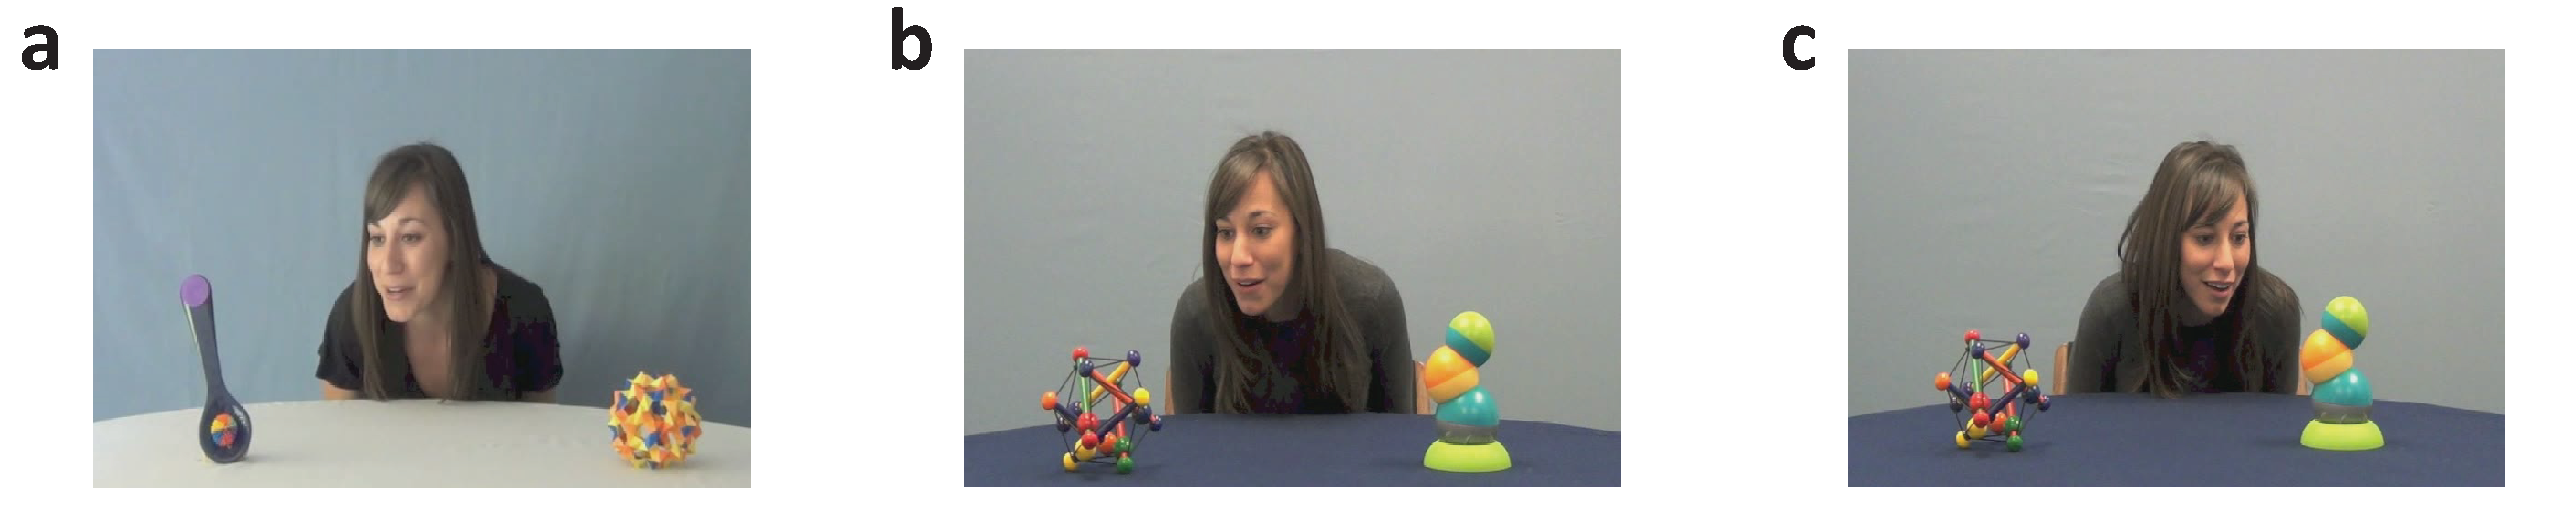
\includegraphics[width=\textwidth]{figures/tri_fig.pdf}}
	\caption{\label{fig:design} Example learning trials from Experiments 1 and 2. In Experiment 1 (a), the speaker turned towards one of the equally-salient toys and labeled it four times over the course of approximately 10 seconds. In Experiment 2, the speaker produced the same social cues and the same label as in Experiment 1, but the target object was either the more perceptually salient toy (b), or the less perceptually salient toy (c). Across experiments, we were thus able to determine the contributions of both salience and social information to early word learning outcomes.}
\end{figure*}

\section{Experiment 1}

In Experiment 1, we set out to measure the development of children's ability to follow and learn from social gaze in the absence of competing salience cues. A na\"{i}ve cue-combination account, in which developmental changes in cue use result from learning their relative predictive weights, should make a null prediction: children's behavior should not change significantly across development. 

Children's eye movements were tracked while they watched a series of naturalistic word-learning videos. In each, children saw a speaker seated at a table between two novel toys. She greeted them, and then turned towards one of the toys and labeled it three times in a short monologue.
After these learning trials children were tested for their knowledge of the referent for the new word using the Looking While Listening procedure \cite{Fernald1998}. In addition, similar test trials were administered for known objects to measure children's processing of familiar words. 

\subsection{Method}

\subsubsection{Stimulus Norming}
Thirty-eight adult participants on Amazon Mechanical Turk were presented the toys two at a time and asked to select the one they would rather play with. Each participant made 20 such choices, with toys sampled at random, producing ~7.6 responses for each pair of toys. Based on these responses, we selected the two toys that were best balanced against each other (see Figure~\ref{fig:design}a).

\subsubsection{Participants}

Parents and their 1--4 year-old children were invited to participate in a short language learning study during their visit to the San Jose Children's Discovery museum. In total, we collected demographic and experimental data from 269 children, 122 of whom were excluded for one or more of the following reasons: abnormal developmental issues ($N= 27$), failure to calibrate ($N=58$), and less than 75\% exposure to English ($N=36$). The final sample consisted of 27 1--1.5 year olds (9 girls), 19 1.5--2 year olds (7 girls), 38 2--2.5 year olds (13 girls), 26 2.5--3 year olds (10 girls), 15 4--3.5 year olds (9 girls), and 22 3.5--4 year olds (11 girls).

\subsubsection{Stimuli}

The experiment consisted of two kinds of trials: learning and test. Learning trials were ~12s video clips in which a speaker first greeted the the child, and then turned towards one of the two toys on the screen, labeling it three times in a short monologue (Figure~\ref{fig:design}a). On the first learning trial, for example, the speaker said ``Hi there! It's a \emph{modi}. Look at the \emph{modi}. What a nice \emph{modi}.''

On each test trial, children saw two objects---one on each side of the screen---and heard a short audio clip of the speaker from the learning trials asking them to find a target object. Each test trial was 7s long, and the target label was heard at ~2.75s. On \emph{Familiar} test trials, both the target and distractor were common objects familiar to young children (e.g. book vs. dog). On \emph{Novel} and  \emph{Mutual Exclusivity (ME)} test trials, children saw both of the toys from the previous learning trials, and were asked to find either the previously named toy (\emph{modi}), or were asked about a novel label (\emph{dax}). These ME trials were designed as a strong test of mapping formation; looking to the correct target on Novel trials could result from familiarity or preference rather than mapping.

In addition, the experiment contained two calibration checks: short videos in which small dancing stars appeared in four places on the screen. Because eye-tracker calibration can be imprecise, especially with younger children \cite{Morgante2011}, this check allowed us to adjust initial calibration settings to minimize the discrepancy between the behavior children produced and the behavior we analyzed \cite<for details, see>{Frank2012d}.

\subsubsection{Design and Procedure}

The two kinds of trials were designed to measure both how children allocate their attention over the course of learning from a social partner, and what word-object mapping information they extract from these learning events. Consequently, in addition to testing children's ability to correctly fixate the target object on Novel trials,in which they heard the label introduced during learning trials, we measured their fixation behavior when they saw the same objects but were asked to find the referent of a novel word. These Mutual Exclusivity (ME) trials provide a strong measure of children's word learning, because above-chance looking on novel trials could be result of a salience preference rather than a mapping between the word and object.

The eye-tracker was first calibrated for each child using a 2-point calibration. Next, children saw four learning trials in which the speaker produced the novel label and disambiguated her target of reference with social gaze. Finally, children saw all of the test trials, in which their knowledge of both familiar and novel word-object mappings was tested. Two calibration checks (described above) were embedded in the learning phase. The entire experiment consisted of 4 learning trials, 8 Familiar, 6 Novel, and 6 ME test trials.

\subsubsection{Data Analysis}

Children's eye movements during both learning and testing were analyzed using a Regions of Interest (ROI) approach. On learning trials, bounding-box ROIs were drawn by a human coder frame-by-frame for the speaker's face and for the two objects. On test trials, a bound-box ROI was drawn for each of the two static images. Children's calibrations were adjusted by fitting a robust linear regression for their fixations during calibration check videos and using this model to transform eye movements during the rest of the experiment \cite{Frank2012d}.

Children's learning and test behaviors were quantified by measuring their proportion of looking to each ROI on each trial. To ensure that proportions were representative, individual test trials were excluded from analysis if eye gaze data was missing for more than half of their duration. 
To compute age-group looking proportions, proportions were computed first for each individual trial, averaged at the individual-child level, and then averaged across children.

Window-of-analysis selection began by coding the point of disambiguation for each trial. This was the onset of the target label for test trials, and the rotation of the speaker's head for learning trials (marked `0' in the graphs in the Results section). The window for each trial began 1s after this point of disambiguation to allow children of all ages enough time to process and continued out to 3s after this point on both learning and test trials. To quantify learning with standard analyses, we aggregated these patterns of looking over time to compute proportion of target looking on each test trial. 

\subsection{Results}

First, in line with the cue-combination account, children were attentive to social cues during learning at all ages measured. For all age groups, looks to both target and distractor made up the minority of children's dwell times. Instead, children in all age groups spent more than 50\% of their time attending to the speaker's face (Figure~\ref{fig:exp1_train}). Second, children were successful at attending to and following the speaker's social gaze even from the youngest ages measured. Children of all ages spent more time looking at the target than at the competitor during learning trials (smallest $t(23)  = 3.20$, $p < .01$).

Also in line with the cue-combination account, Analyses of test trials showed broad success on Familiar, Novel, and ME trials across development. The 1--1.5 year-olds trended towards significance on familiar trials ($t(26)  = 1.65$, $p = .11$), and were non-significantly in the correct direction on Novel and ME trials. At all other ages, children looked to the target at above-chance levels on all test trials (smallest $t(17)  = 2.10$, $p = .05$). 

However, children's abilities both to follow social cues during learning trials and to find the correct target on test trials improved across development. To quantify this improvement, we fit a mixed effects logistic regression to the data \cite{Jaeger2008}. This analysis revealed significant improvement across age ($\beta = .61$, $z = 4.03$, $p <.001$), as well a significant significant effect of Learning as compared to Novel trials ($\beta = 1.18$, $z = 3.11$, $p <.01$). No other effects or interactions approached significance. Figure~\ref{fig:exp1_train_test} shows proportion of looking all kinds of trials at all ages.

 \begin{figure}[t]
	\center{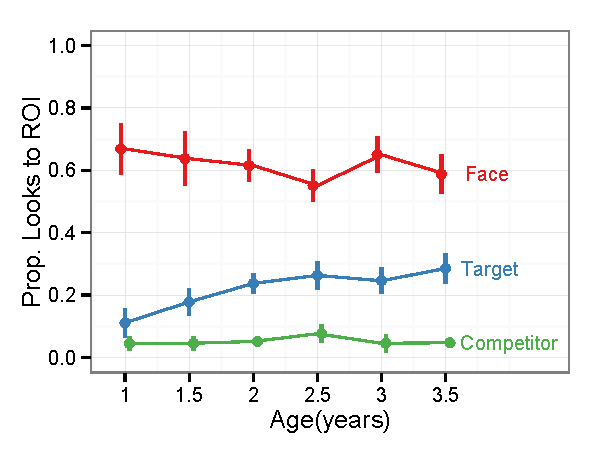
\includegraphics[width=.5\textwidth]{figures/exp1_train.pdf}}
	\caption{\label{fig:exp1_train} Proportion of fixations directed to the target and to the speaker's face during learning trials. Children of all ages spent the majority of the learning trials fixating the speaker's face, but disengaging from the face and fixating the target increased across development. Shaded regions indicate $\pm$1SE.}
\end{figure}

\begin{figure}[!t]
	\center{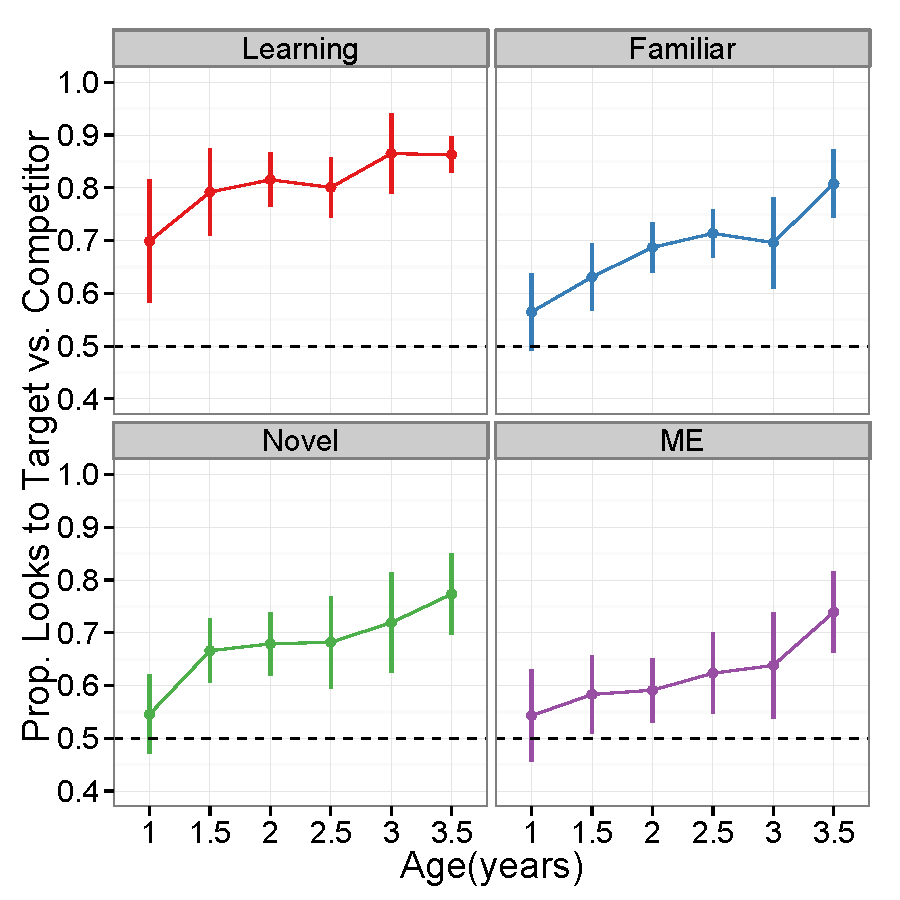
\includegraphics[width=.45\textwidth]{figures/exp1_train_test.pdf}}
	\caption{\label{fig:exp1_train_test} Proportion of time children fixated the correct correct target on each type of test trial in Experiment 1. Children improved on all measures across development. Each dot indicates one half-year age group and each line represents a 95\% confidence interval computed by non-parametric bootstrap. A proportion of .5 indicates chance performance.}
\end{figure}	

\subsection{Discussion}

Together, these results provide evidence both of early competence in the use of social gaze to determine the target of a speaker's reference, as well as improvement across development. Further, improvements in gaze-following also paralleled improvements in both finding the referents of these novel words on subsequent learning trials, and also finding the referents of familiar words (Figure~\ref{fig:exp1_train_test}).

These results thus provide support for one key claim of the developmental cue-combination account: children are sensitive to social cues quite early. Young children could assign  small---but non-zero---weight to social cues, and then gradually assign them more credibility over development. However, the results provide strong evidence \emph{against} the prediction that developmental change is due to relative re-weighting for two reasons. First, children of all ages found the speaker's face highly engaging, and spent the majority of their time fixating it rather than the referents on learning trials. The primary behavioral development was the ability to disengage from the speaker's face. Second, children showed gradual improvement in fixating the target during both learning and test trials well into their fourth year.

This data could be consistent with a modified version of the cue-combination account in which cues both change in their individual weights and in their relative weights due to learning. However, while children undeniably encounter naming events in their third and fourth years, it would seem unlikely that the process of learning the cue validity of social gaze would extend over such a long period of time. 

In Experiment 2 we manipulated the relative salience of the target and distractor objects to which children were exposed. This allowed us to test two further predictions of the na\"{i}ve cue-combination account: that salience plays a strong role in directing the attention of young word-learners, and that salient objects draw more attention than social cues.

\section{Experiment 2}

Experiment 2 was identical to Experiment 1 in all respects except for the identity of the novel toys that served as the target and distractor. In contrast to Experiment 1, in which the two toys were balanced in their visual salience, the two toys in Experiment 2 were mismatched. For children in the \emph{Salient} condition, the target was the more interesting toy, and the distractor the less interesting toy. In the \emph{Non-Salient} condition, the identities of the toys were switched---the target was the less salient toy. Thus, Experiment 2 allows us to investigate children's use of social cues to learn new words when they are aligned with salience, and when they are in opposition \cite<as in>{Hollich2000,Pruden2006}.

\subsection{Method}

\subsubsection{Participants}

Participants were recruited from the floor of the San Jose Children's Discovery museum as in Experiment 1. This time, however, we focused on the three youngest age groups. In the Salience condition, demographic and experimental data were collected from 117 children, 52 of whom were excluded for one or more of the following reasons: abnormal developmental issues ($N= 13$), failure to calibrate ($N=25$), less than 75\% exposure to English ($N=33$), and inattentiveness ($N=2$). The final sample consisted of 22 1-1.5 year olds (11 girls), 21 1.5-2 year olds (10 girls), 19 2-2.5 year olds (9 girls). In the Non-Salience condition, data were collected from 126 children, 71 of whom were excluded for one or more of the following reasons: abnormal developmental issues ($N= 9$), failure to calibrate ($N=26$), and less than 75\% exposure to English ($N=36$). The final sample consisted of 26 1-1.5 year olds (13 girls), 25 1.5-2 year olds (11 girls), 15 2-2.5 year olds (4 girls).

\subsubsection{Stimuli, Design, and Procedure}

Experimental stimuli were identical to those in Experiment 1, except that the identities of the novel toys were changed and new videos were recorded. The procedure, including the order of the trials, was identical.

\subsection{Results and Discussion}
\begin{figure}[!t]
	\center{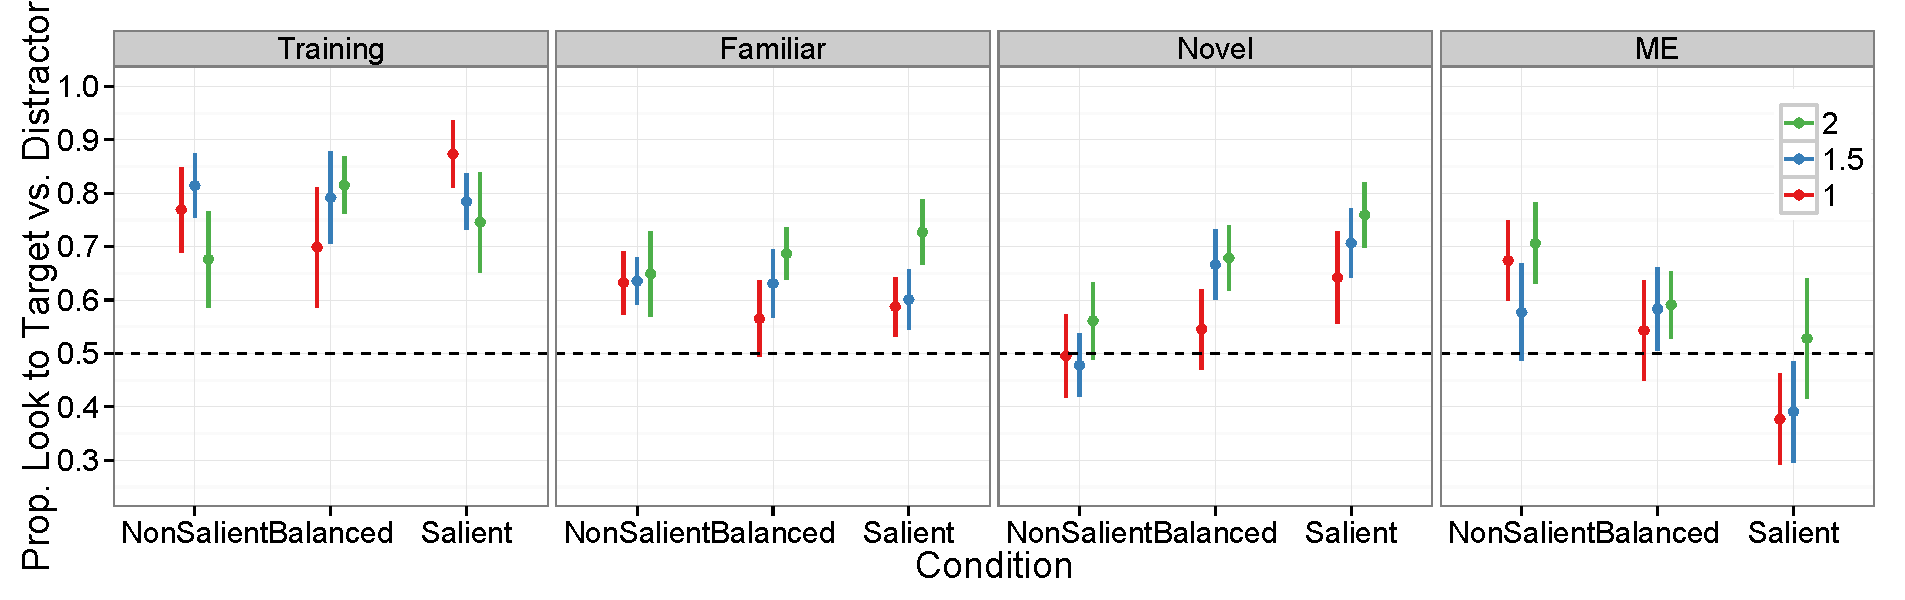
\includegraphics[width=.45\textwidth]{figures/exp1_2_train_test.pdf}}
	\caption{\label{fig:exp1_2} Proportion of time children fixated the correct correct target on Learning and Test trials in Experiments 1 and 2. Salience played a large role in affecting looking behavior at test, but relatively little during learning. Each dot indicates one half-year age group and each line represents a 95\% confidence interval computed by non-parametric bootstrap. A proportion of .5 indicates chance performance.}
\end{figure}


\begin{table}[b]
\begin{center} 
\caption{Mixed-effects Regression Coefficients Predicting Looking Behavior in Experiments 1 and 2.} 
\label{tab:model_table} 
\vskip 0.12in
\begin{tabular}{l r r r l} 
\hline
Predictor  &  Value (SE) & \emph{t}-value & Sig.\\
\hline
Intercept  & -.65 (.63) & -1.04 & $p = .3$&\\
Age (yrs) & .42 (.27) &  1.58 & $p = .11$&\\
Familiar & 1.55 (.73) & 2.13 & $p < .05$&*\\
Salient  & .96 (.48) & 1.98 & $p < .05$&*\\
NonSalient  & -.97 (.37) & -2.63 & $p < .01$&**\\
Learning & 1.55 (.73) & 2.13 & $p < .05$& *\\
ME & -.29 (.36) & -.80 & $p =.42$&\\
Salient*Learn  & -.03 (.84) & -.035 & $p = .97$&\\
NonSal*Learn & 1.09 (.65) & -1.65 & $p = .85$&\\
Sal*ME & -2.28 (.61) & -3.73 & $p = -.09$&.\\
NonSal*ME  & 1.67 (.54) & 3.07 & $p < .01$&**\\
\hline
\end{tabular} 
\end{center} 
\end{table}

To determine the effect of perceptual salience on word learning, we compared children's looking in the Salient and Non-Salient conditions not only to each other, but also to the Balanced condition in Experiment 1. The nai\"{i}ve cue combination accounts makes two predictions: (1) there should be an effect of salience during learning trials, and (2) this effect should diminish over the course of development.

First, in contrast to the prediction of the na\"{i}ve cue-combination account, children's looking behavior during learning trials was not significantly affected by the salience of the target and distractor. As in Experiment 1, children of all ages spent the more time looking at the target than the distractor, but looking time to both made up the minority of their dwell time; children spent the majority of learning trials looking at the speaker's face (DOES THIS NEED A FIGURE?).

This null-result could be due to the toys being too similar in their salience, making this a weak est of the cue-combination model. However, salience exerted a strong effect on test trials---children in all age groups were strongly attracted to the salient object. When the target referent was salient, children at all ages looked at it for the majority of the window of analysis on Novel test trials (smallest $t(19)  = 2.96$, $p < .01$). When the target was non-salient, no age group look showed evidence of learning on Novel test trials (largest $t(13)  = 1.46$, $p = .17$). Mutual-exclusivity (ME) trials showed the opposite pattern. When the target referent was salient, children in the two younger age groups looked at the correct referent on ME trials (the competitor) at \emph{below} chance levels (smallest $t(20) = -2.29$, $p < .05$). In the Non-Salient condition, even the youngest children looked at the correct referent on ME trials at above chance levels (smallest $t(22) = 4.51$, $p < .001$). Figure~\ref{fig:exp1_2}) shows looking behavior in both Experiments 1 and 2 together.

To test the second prediction, we fit a mixed-effects logistic regression to the data from all three experiments to determine how how age and experimental condition impacted looking behavior in training and test. After controlling for performance on Familiar trials, this regression showed a significant effect of condition, and an interaction between trial type and condition. Children looked more to the salient object at test regardless of whether it was the target or distractor, and significantly more at the target during learning trials regardless of whether it was salient. Further, there was no interaction of any of these factors with age (Table~\ref{tab:model_table}). 

Together with the t-tests above, this analysis suggests that children are not learning to relative weights on salience and social cues over the course of development. While salience certainly plays a role in directing looking behavior, it does not appear to play a role during learning itself. Instead, salience appears to have a strong effect during test. In the absence of any social information, salience directs children's attention in a way that does not appear to change over early development.

\section{Conclusion}

Main ideas: face is relevant, attended to, and used to find the target. The reason why could change over development (e.g. face itself could be salient), but either way ``social cues'' get used.

Salience definitely matters, but mostly at test. Could be a cue-weighting model in which once the face is gone the salience cue gets high weight. But something about cue weighting seems wrong based on learning trial behavior. Unclear how to predict developmental differences unless cues are not normalized. Also, in general, this kind of model really misses the inherent temporal aspects of word learning.

Salience could still be used in the absence of social information for either smart or dumb reasons, and might end up being adaptive. But it seems pretty clear that we're not seeing a re-weighting across development of these two cues.

Seems like what we really want to pay attention to are memory, attentional control, and timing. Probably all of these are developing?

Maybe the two timescales idea \cite{Frank2009a,McMurray2012} is the right way to think about this kind of thing. Performing above competence? 

\section{Acknowledgments}

We are grateful to Janelle Klaas for collecting the data, and to  all of the members of the Language and Cognition Lab for their feedback on this project. In addition, we thank the parents, children, and staff at the San Jose Children's Discovery Museum for supporting us in collecting developmental data. This work was supported by a NIH NRSA F32HD075577 to DY as well as grants from the Merck Scholars Foundation and the Stanford Center Health Research Initiative to MCF.

\newpage

\bibliographystyle{apacite}

\setlength{\bibleftmargin}{.125in}
\setlength{\bibindent}{-\bibleftmargin}

\bibliography{library11}


\end{document}
